 \begin{figure*}[ht]
\centering
\begin{subfigure}{.31\linewidth}
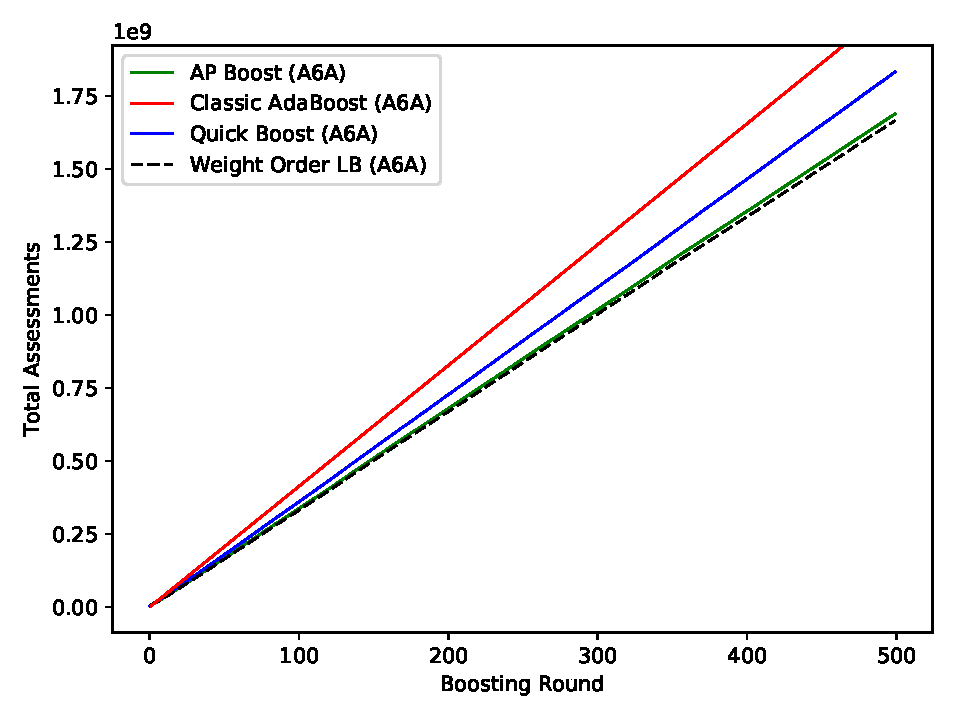
\includegraphics[width=\linewidth]{decisiontree/figures/result3_wolb_a6a}
\end{subfigure}
\begin{subfigure}{.31\linewidth}
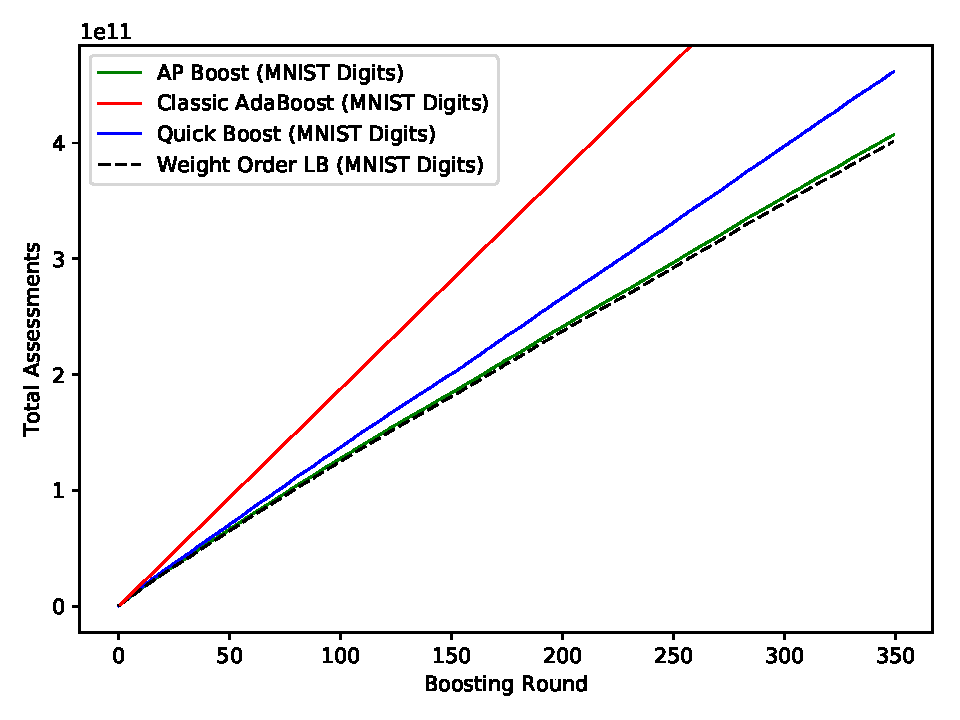
\includegraphics[width=\linewidth]{decisiontree/figures/result3_wolb_mnist}
\end{subfigure}
\begin{subfigure}{.31\linewidth}
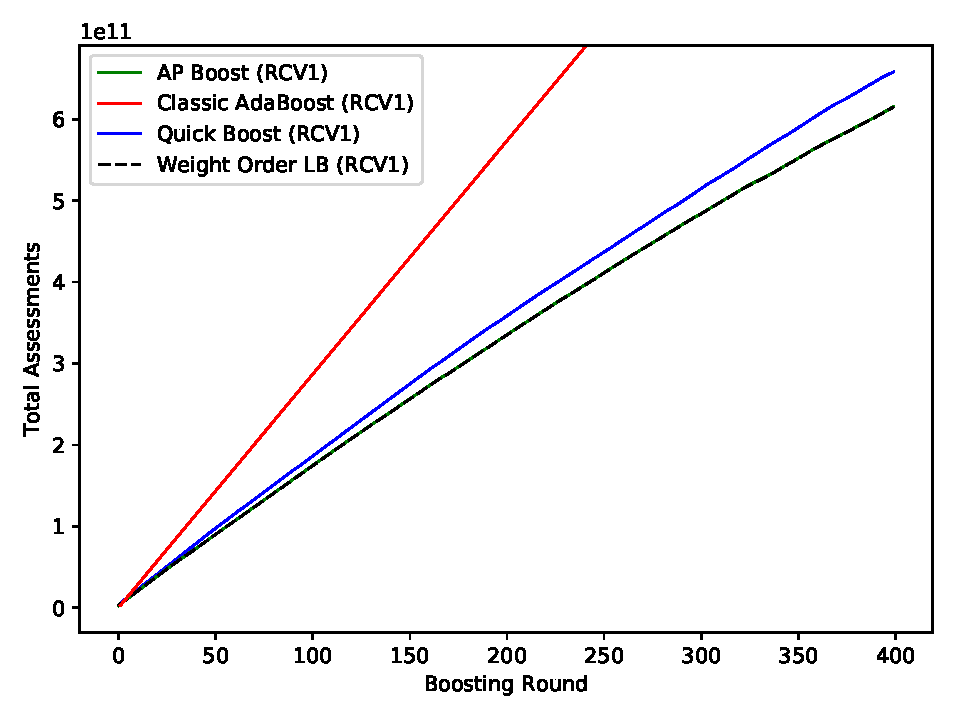
\includegraphics[width=\linewidth]{decisiontree/figures/result3_wolb_rcv1}
\end{subfigure}
\begin{subfigure}{.31\linewidth}
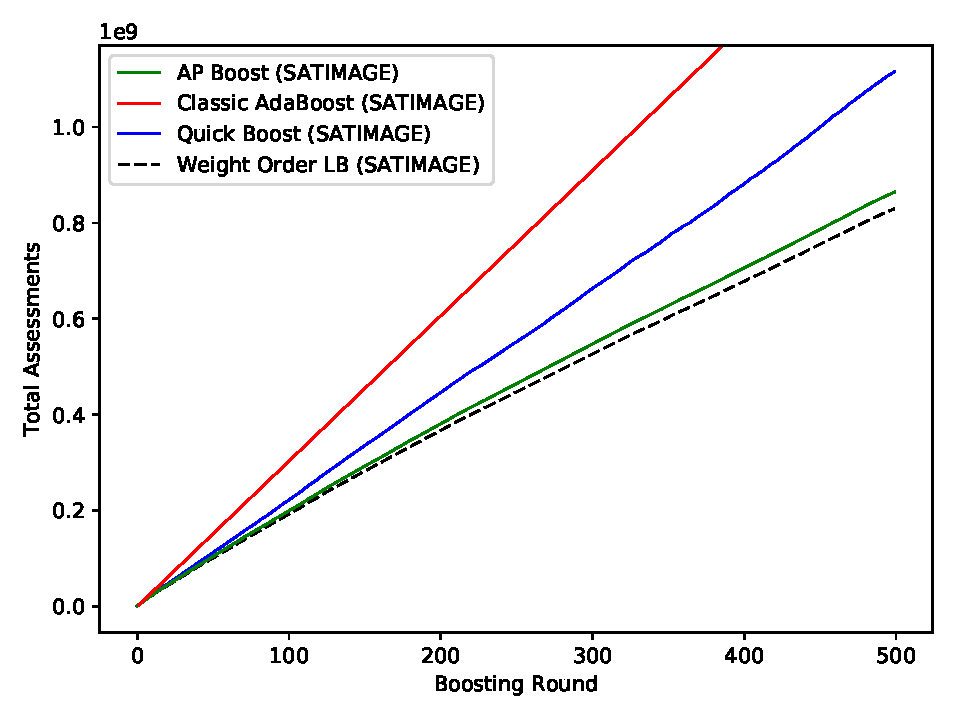
\includegraphics[width=\linewidth]{decisiontree/figures/result3_wolb_satimage}
\end{subfigure}
\begin{subfigure}{.31\linewidth}
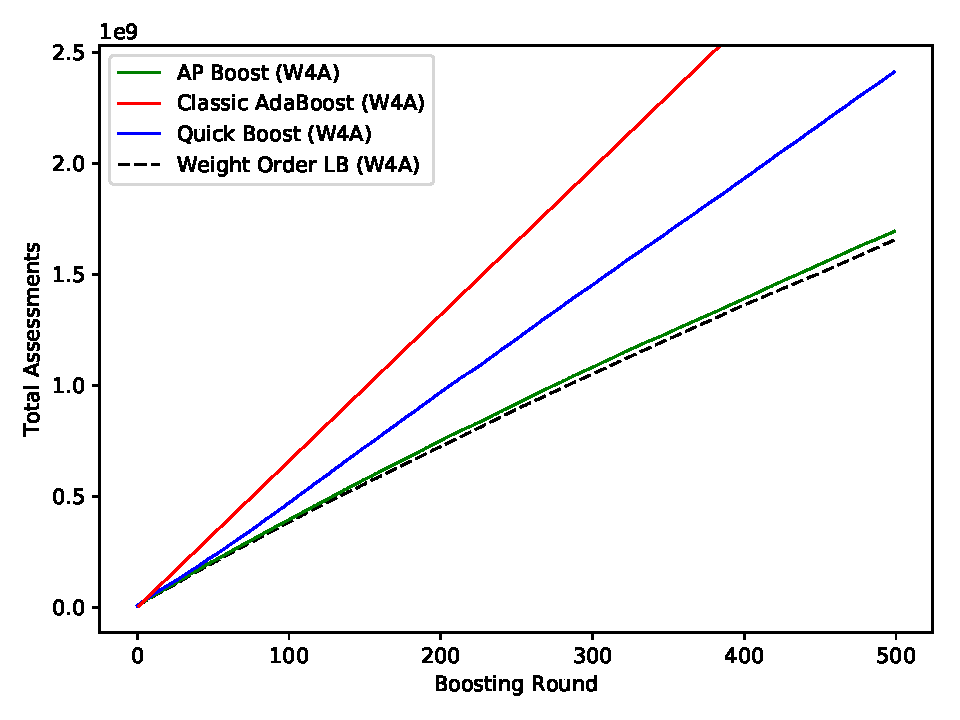
\includegraphics[width=\linewidth]{decisiontree/figures/result3_wolb_w4a}
\end{subfigure}
\caption{We report the total number of assessments at various boosting rounds used by the algorithms, as well as the weight order lower bound. In all of these experiments, our algorithm, \texttt{AP Boost}, not only consistently beats \texttt{Quick Boost} but it also almost matches the lower bound.}
\label{fig:wolb}
\end{figure*}